\documentclass[a4paper, openany]{memoir}

\usepackage[utf8]{inputenc}
\usepackage[T1]{fontenc} 
\usepackage[english]{babel}

\usepackage{fancyhdr}
\usepackage{float}

\usepackage{amsmath}
\usepackage{amsthm}
\usepackage{amssymb}
\usepackage{enumitem}
\usepackage{multicol}
\usepackage[bookmarksopen=true,bookmarksopenlevel=2]{hyperref}
\usepackage{tikz}
\usepackage{listings}
\usepackage{xcolor}
\usepackage{indentfirst}
\usepackage{caption}
\usepackage{subcaption}

\pagestyle{fancy}
\fancyhf{}
\fancyhead[LE]{\leftmark}
\fancyhead[RO]{\rightmark}
\fancyhead[RE, LO]{Algorithmics II}
\fancyfoot[LE, RO]{\thepage}
\fancyfoot[RE, LO]{Pete Gautam}

\usetikzlibrary{positioning, automata, arrows}

\definecolor{codegreen}{rgb}{0,0.6,0}
\definecolor{codegray}{rgb}{0.5,0.5,0.5}
\definecolor{codepurple}{rgb}{0.58,0,0.82}
\definecolor{backcolour}{rgb}{0.95,0.95,0.92}

\lstdefinestyle{thestyle}{
    backgroundcolor=\color{backcolour},
    basicstyle=\ttfamily\footnotesize,
    keywordstyle=\color{red!80}\bfseries,
    ndkeywordstyle=\color{blue!80}\bfseries,
    identifierstyle=\color{black},
    commentstyle=\color{codegreen},
    stringstyle=\color{codepurple},
    breakatwhitespace=false,
    breaklines=true,
    captionpos=b,
    keepspaces=true,
    numberstyle=\tiny\color{codegray},
    numbers=left,
    numbersep=2pt,
    showspaces=false,
    showstringspaces=false,
    showtabs=false,          
    tabsize=2
}

\lstdefinelanguage{pseudocode}{ 
    keywords={new, return, this, null, if, in, while, else, for, get, set, class, and, or, not, range},
    ndkeywords={int, char, bool, void, double, true, false, Line, LineSegment, Point, Rectangle, List, Map, BTree, BNode, VLine, HLine},
    sensitive=true,
    comment=[l]{//},
    morecomment=[s]{/*}{*/},
    morestring=[b]',
    morestring=[b]"
}

\lstset{style=thestyle}

\usetikzlibrary{shapes, positioning}

\chapterstyle{thatcher}

\setcounter{chapter}{1}

\begin{document}
    \chapter{String and Text Algorithms}
    \section{Suffix Tries and Trees}
    In this section, we will look at suffix tries and trees, and how they can be used to efficiently perform different string operations. We begin by defining some terminologies:
    \begin{itemize}
        \item an \emph{alphabet} consists of all letters that a string can be composed of, e.g. ASCII. It is denoted by $\Sigma$.
        \item a \emph{string} is a word on the alphabet.
        \item the \emph{length} of a string $S$ is the number of letters it has.
        \item for a string $S$, we use $S[i]$ to denote the $i$-th character in the string.
        \item for a string $S$, we use $S[i:j]$ to denote the substring of $S$ from position $i$ to $j$ (both included).
        \item for strings $S$ and $T$, their \emph{concatenation} is denoted by $ST$.
        \item the \emph{empty string} is denoted by $\epsilon$. It has length $0$.
        \item for a string $S$, another string $U$ is a \emph{substring} of $T$ if $S = TUV$, for strings $T$ and $V$.
        \item for two strings $S$ and $T$, we say that $U$ is a \emph{common substring} if it is a substring of both $S$ and $T$.
        \item for a string $S$, a \emph{subsequence} of $S$ is composed of characters in $S$ (in the given order), but it need not be a continuous block like a substring. We can delete characters from $S$ to get a subsequence.
        \item for strings $S$ and $T$, we say that $U$ is a \emph{common subsequence} if it is a subsequence of both $S$ and $T$.
        \item for a string $S$, a \emph{prefix} is a substring starting from the start.
        \item for a string $S$, a \emph{suffix} is a substring ending at the end.
        \item for an alphabet $\Sigma$, the set $\Sigma^*$ is composed of all strings on $\Sigma$, including the empty string $\epsilon$.
        \item a \emph{leaf node} in a tree has no children.
        \item a \emph{branch node} in a tree has at least one child.
        \item a \emph{unary node} in a tree has precisely one child.
        \item a \emph{binary node} in a tree has precisely two children.
    \end{itemize}

    We have previously seen suffix tries used to search hundreds of substrings in a single long text. We can do this using KMP or BM, but these are linear in terms of the long text during each computation. We can use suffix tries to make the algorithm to process the long text just once, and linear in terms of the number of strings we have to search. This is because the trie pre-processes the text and creates an index for it. Because the text is typically much longer than the substrings, this is much faster in practice.

    \subsection{Longest repeated and common substring}
    Given a string $S$, we want to compute the longest repeated substring in $S$. A naive solution for this will loop through the starting position of the first repeat and the second repeat, and check whether there is a match of some length- this takes $O(n^3)$ time. We can use a dynamic programming algorithm to make the algorithm more efficient.

    In the algorithm, we store the characters of the string as both rows and columns. If there is a match at a cell, we make the entry 1; otherwise, the entry is 0. The longest common substring corresponds to the greatest sum we can produce when we traverse the long diagonals. The following example illustrates this algorithm to find the longest repeated substring of \texttt{ababa}:
    \begin{table}[H]
        \centering
        \begin{tabular}{c|ccccc}
            & \texttt{a} & \texttt{b} & \texttt{a} & \texttt{b} & \texttt{a} \\
            \hline
            \texttt{a} & - & 0 & {\color{red}1} & 0 & 1 \\
            \texttt{b} & - & - & 0 & {\color{red}1} & 0 \\
            \texttt{a} & - & - & - & 0 & {\color{red}1} \\
            \texttt{b} & - & - & - & - & 0 \\
            \texttt{a} & - & - & - & - & -
        \end{tabular}
    \end{table}
    \noindent We only compute the entries on the right side of the diagonal as the values are symmetric. There is always a match at the diagonal- we are not interested in that. In this case, the longest repeated substring is \texttt{aba}. Note that the value \texttt{a} is shared between the two substrings- this is allowed because the index of the matching \texttt{a} is still different. 

    % TODO: Add algorithm
    This algorithm has complexity $O(n^2)$ in both time and space.
    
    We can easily modify this dynamic programming algorithm to compute the longest common substring of two strings. The following example illustrates this.
    \begin{table}[H]
        \centering
        \begin{tabular}{c|ccccc}
            & \texttt{a} & \texttt{b} & \texttt{c} & \texttt{a} & \texttt{b} \\
            \hline
            \texttt{b} & 0 & 1 & 0 & 0 & 1 \\
            \texttt{b} & 0 & {\color{red}1} & 0 & 0 & 1 \\
            \texttt{c} & 0 & 0 & {\color{red}1} & 0 & 0 \\
            \texttt{a} & 1 & 0 & 0 & {\color{red}1} & 0 \\
            \texttt{a} & 1 & 0 & 0 & 1 & 0
        \end{tabular}
    \end{table}
    \noindent In this case, we need to compute both sides of the diagonal, and the diagonal, since the two strings are assumed to be different. Here, the longest common substring is \texttt{bca}.

    % TODO: Add algorithm
    This algorithm has complexity $O(mn)$ in both time and space, where $m$ and $n$ are the lengths of the two strings.

    \subsection{Suffix Tries}
    We will now improve the time (and space) complexity of these algorithms using suffix tries. For a string $S$, the suffix tree of $S$ stores all the suffixes in $S$ including the entire string. Using this representation, we can compute the longest repeated substring in $O(n)$ time and longest common substring in $O(m+n)$ time. Moreover, we can search multiple strings (whose sum of length is $r$) in $O(n+r)$ time.

    A trie is a branching tree that is used to store strings in an alphabet. It has the following properties:
    \begin{itemize}
        \item a trie has a root vertex;
        \item every edge in the trie corresponds to a character from the alphabet;
        \item no two children of a branch node have the same edge label;
        \item every node corresponds to a string in the alphabet, which is given by traversing the tree from the root to the given node;
        \item every node is marked in a way to recognise whether it corresponds to one of the given words.
    \end{itemize}
    An example of the trie on the words- \texttt{arch}, \texttt{are}, \texttt{area}, \texttt{the}, \texttt{there} and \texttt{these} is given below:
    \begin{figure}[H]
        \centering
        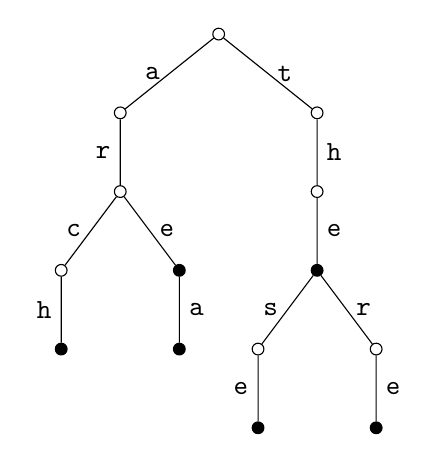
\begin{tikzpicture}[
            level distance=1cm,
            level 1/.style={sibling distance=2.5cm},
            level 2/.style={sibling distance=2cm},
            level 3/.style={sibling distance=1.5cm},
        ]
            \node[circle, draw, inner sep=1.5pt] {}
            child {
                node[circle, draw, inner sep=1.5pt] {}
                child {
                    node[circle, draw, inner sep=1.5pt] {}
                    child {
                        node[circle, draw, inner sep=1.5pt] {}
                        child {
                            node[circle, draw, fill, inner sep=1.5pt] {}
                            edge from parent node[left] {\texttt{h}}
                        }
                        edge from parent node[left] {\texttt{c}}
                    }
                    child {
                        node[circle, draw, fill, inner sep=1.5pt] {}
                        child {
                            node[circle, draw, fill, inner sep=1.5pt] {}
                            edge from parent node[right] {\texttt{a}}
                        }
                        edge from parent node[right] {\texttt{e}}
                    }
                    edge from parent node[left] {\texttt{r}}
                }
                edge from parent node[left] {\texttt{a}}
            }
            child {
                node[circle, draw, inner sep=1.5pt] {}
                child {
                    node[circle, draw, inner sep=1.5pt] {}
                    child {
                        node[circle, draw, fill, inner sep=1.5pt] {}
                        child {
                            node[circle, draw, inner sep=1.5pt] {}
                            child {
                                node[circle, draw, fill, inner sep=1.5pt] {}
                                edge from parent node[left] {\texttt{e}}
                            }
                            edge from parent node[left] {\texttt{s}}
                        }
                        child {
                            node[circle, draw, inner sep=1.5pt] {}
                            child {
                                node[circle, draw, fill, inner sep=1.5pt] {}
                                edge from parent node[right] {\texttt{e}}
                            }
                            edge from parent node[right] {\texttt{r}}
                        }
                        edge from parent node[right] {\texttt{e}}
                    }
                    edge from parent node[right] {\texttt{h}}
                }
                edge from parent node[right] {\texttt{t}}
            };
        \end{tikzpicture}
    \end{figure}
    \noindent We mark by black any node that corresponds to a string.

    A suffix trie is a trie that stores all the suffixes of a given string. For example, the suffix trie of \texttt{queue} is given below.
    \begin{figure}[H]
        \centering
        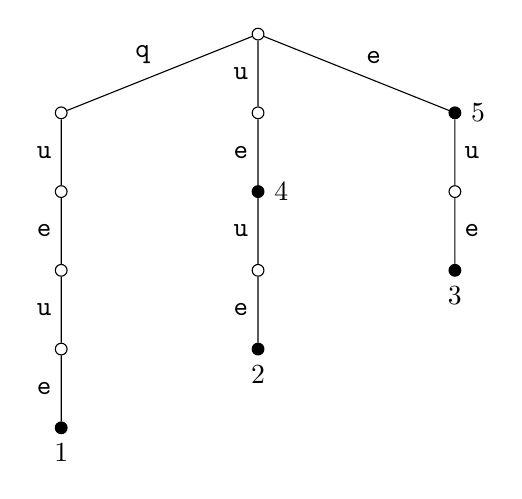
\begin{tikzpicture}[
            level distance=1cm,
            level 1/.style={sibling distance=2.5cm},
            level 2/.style={sibling distance=2cm},
            level 3/.style={sibling distance=1.5cm},
        ]
            \node[circle, draw, inner sep=1.5pt] {}
            child {
                node[circle, draw, inner sep=1.5pt] {}
                child {
                    node[circle, draw, inner sep=1.5pt] {}
                    child {
                        node[circle, draw, inner sep=1.5pt] {}
                        child {
                            node[circle, draw, inner sep=1.5pt] {}
                            child {
                                node[circle, fill, draw, inner sep=1.5pt, label={-90:1}] {}
                                edge from parent node[left] {\texttt{e}}
                            }
                            edge from parent node[left] {\texttt{u}}
                        }
                        edge from parent node[left] {\texttt{e}}
                    }
                    edge from parent node[left] {\texttt{u}}
                }
                edge from parent node[above left] {\texttt{q}}
            }
            child {
                node[circle, draw, inner sep=1.5pt] {}
                child {
                    node[circle, fill, draw, inner sep=1.5pt, label={0:4}] {}
                    child {
                        node[circle, draw, inner sep=1.5pt] {}
                        child {
                            node[circle, fill, draw, inner sep=1.5pt, label={-90:2}] {}
                            edge from parent node[left] {\texttt{e}}
                        }
                        edge from parent node[left] {\texttt{u}}
                    }
                    edge from parent node[left] {\texttt{e}}
                }
                edge from parent node[left] {\texttt{u}}
            }
            child {
                node[circle, fill, draw, inner sep=1.5pt, label={0:5}] {}
                child {
                    node[circle, draw, inner sep=1.5pt] {}
                    child {
                        node[circle, fill, draw, inner sep=1.5pt, label={-90:3}] {}
                        edge from parent node[right] {\texttt{e}}
                    }
                    edge from parent node[right] {\texttt{u}}
                }
                edge from parent node[above right] {\texttt{e}}
            };
        \end{tikzpicture}
    \end{figure}
    \noindent For a suffix trie, we also want each suffix to end at a leaf node. This is not the case in the trie above- the suffixes \texttt{ue} and \texttt{e} end at branch nodes. This is because there is a suffix (\texttt{ue}) that is a prefix of another one (\texttt{ueue}). To fix this issue, we add a unique termination symbol \texttt{\$} that is not present in the alphabet. This ensures that no suffix is a prefix of another suffix. In this case, the suffix trie for \texttt{queue} is the following:
    \begin{figure}[H]
        \centering
        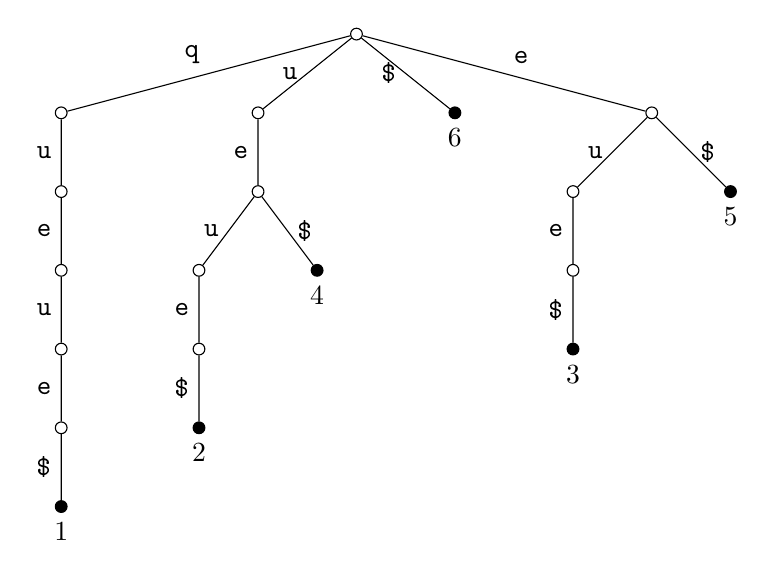
\begin{tikzpicture}[
            level distance=1cm,
            level 1/.style={sibling distance=2.5cm},
            level 2/.style={sibling distance=2cm},
            level 3/.style={sibling distance=1.5cm},
        ]
            \node[circle, draw, inner sep=1.5pt] {}
            child {
                node[circle, draw, inner sep=1.5pt] {}
                child {
                    node[circle, draw, inner sep=1.5pt] {}
                    child {
                        node[circle, draw, inner sep=1.5pt] {}
                        child {
                            node[circle, draw, inner sep=1.5pt] {}
                            child {
                                node[circle, draw, inner sep=1.5pt] {}
                                child {
                                    node[circle, fill, draw, inner sep=1.5pt, label={-90:1}] {}
                                    edge from parent node[left] {\texttt{\$}}
                                }
                                edge from parent node[left] {\texttt{e}}
                            }
                            edge from parent node[left] {\texttt{u}}
                        }
                        edge from parent node[left] {\texttt{e}}
                    }
                    edge from parent node[left] {\texttt{u}}
                }
                edge from parent node[above left] {\texttt{q}}
            }
            child {
                node[circle, draw, inner sep=1.5pt] {}
                child {
                    node[circle, draw, inner sep=1.5pt] {}
                    child {
                        node[circle, draw, inner sep=1.5pt] {}
                        child {
                            node[circle, draw, inner sep=1.5pt] {}
                            child {
                                node[circle, fill, draw, inner sep=1.5pt, label={-90:2}] {}
                                edge from parent node[left] {\texttt{\$}}
                            }
                            edge from parent node[left] {\texttt{e}}
                        }
                        edge from parent node[left] {\texttt{u}}
                    }
                    child {
                        node[circle, fill, draw, inner sep=1.5pt, label={-90:4}] {}
                        edge from parent node[right] {\texttt{\$}}
                    }
                    edge from parent node[left] {\texttt{e}}
                }
                edge from parent node[left] {\texttt{u}}
            }            
            child {
                node[circle, fill, draw, inner sep=1.5pt, label={-90:6}] {}
                edge from parent node[left] {\texttt{\$}}
            }
            child {
                node[circle, draw, inner sep=1.5pt] {}
                child {
                    node[circle, draw, inner sep=1.5pt] {}
                    child {
                        node[circle, draw, inner sep=1.5pt] {}
                        child {
                            node[circle, fill, draw, inner sep=1.5pt, label={-90:3}] {}
                            edge from parent node[left] {\texttt{\$}}
                        }
                        edge from parent node[left] {\texttt{e}}
                    }
                    edge from parent node[left] {\texttt{u}}
                }
                child {
                    node[circle, fill, draw, inner sep=1.5pt, label={-90:5}] {}
                    edge from parent node[right] {\texttt{\$}}
                }
                edge from parent node[above right] {\texttt{e}}
            };
        \end{tikzpicture}
    \end{figure}

    We will now use the suffix trie above to find \texttt{ue}. We use the suffix trie to descend from the root to the branch corresponding to the character \texttt{u}.
    \begin{figure}[H]
        \centering
        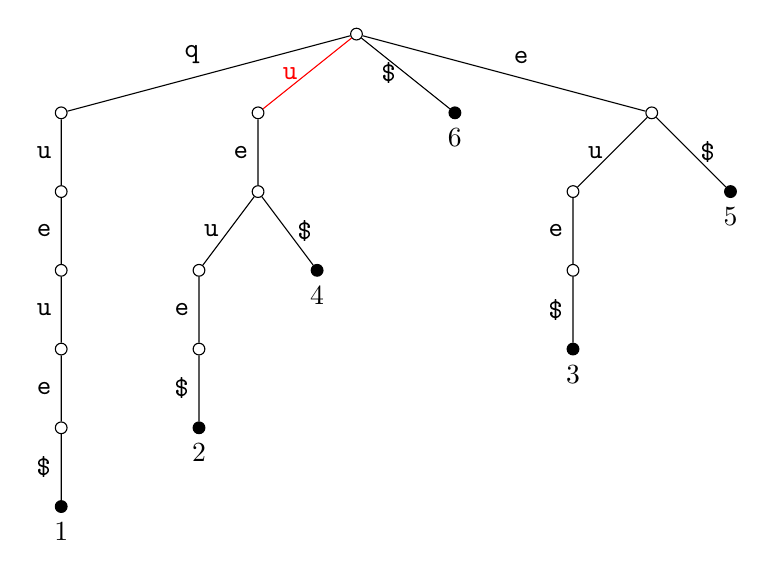
\begin{tikzpicture}[
            level distance=1cm,
            level 1/.style={sibling distance=2.5cm},
            level 2/.style={sibling distance=2cm},
            level 3/.style={sibling distance=1.5cm},
        ]
            \node[circle, draw, inner sep=1.5pt] {}
            child {
                node[circle, draw, inner sep=1.5pt] {}
                child {
                    node[circle, draw, inner sep=1.5pt] {}
                    child {
                        node[circle, draw, inner sep=1.5pt] {}
                        child {
                            node[circle, draw, inner sep=1.5pt] {}
                            child {
                                node[circle, draw, inner sep=1.5pt] {}
                                child {
                                    node[circle, fill, draw, inner sep=1.5pt, label={-90:1}] {}
                                    edge from parent node[left] {\texttt{\$}}
                                }
                                edge from parent node[left] {\texttt{e}}
                            }
                            edge from parent node[left] {\texttt{u}}
                        }
                        edge from parent node[left] {\texttt{e}}
                    }
                    edge from parent node[left] {\texttt{u}}
                }
                edge from parent node[above left] {\texttt{q}}
            }
            child {
                node[circle, draw, inner sep=1.5pt] {}
                child {
                    node[circle, draw, black, inner sep=1.5pt] {}
                    child {
                        node[circle, draw, inner sep=1.5pt] {}
                        child {
                            node[circle, draw, inner sep=1.5pt] {}
                            child {
                                node[circle, fill, draw, inner sep=1.5pt, label={-90:2}] {}
                                edge from parent node[left] {\texttt{\$}}
                            }
                            edge from parent node[left] {\texttt{e}}
                        }
                        edge from parent[black] node[left] {\texttt{u}}
                    }
                    child {
                        node[circle, fill, draw, inner sep=1.5pt, label={-90:4}] {}
                        edge from parent node[right] {\texttt{\$}}
                    }
                    edge from parent[black] node[left] {\texttt{e}}
                }
                edge from parent[red] node[left] {\texttt{u}}
            }            
            child {
                node[circle, fill, draw, inner sep=1.5pt, label={-90:6}] {}
                edge from parent node[left] {\texttt{\$}}
            }
            child {
                node[circle, draw, inner sep=1.5pt] {}
                child {
                    node[circle, draw, inner sep=1.5pt] {}
                    child {
                        node[circle, draw, inner sep=1.5pt] {}
                        child {
                            node[circle, fill, draw, inner sep=1.5pt, label={-90:3}] {}
                            edge from parent node[left] {\texttt{\$}}
                        }
                        edge from parent node[left] {\texttt{e}}
                    }
                    edge from parent node[left] {\texttt{u}}
                }
                child {
                    node[circle, fill, draw, inner sep=1.5pt, label={-90:5}] {}
                    edge from parent node[right] {\texttt{\$}}
                }
                edge from parent node[above right] {\texttt{e}}
            };
        \end{tikzpicture}
    \end{figure}
    \noindent We then descend from this branch to the one corresponding to the character \texttt{e}.
    \begin{figure}[H]
        \centering
        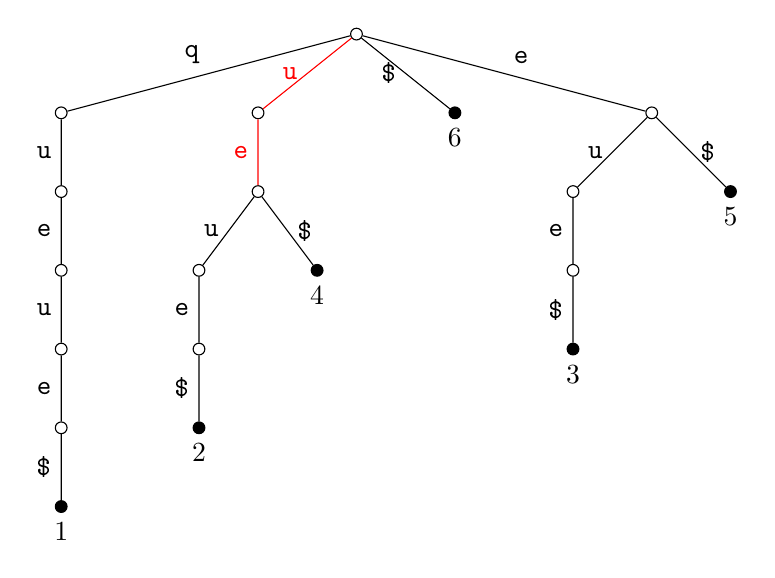
\begin{tikzpicture}[
            level distance=1cm,
            level 1/.style={sibling distance=2.5cm},
            level 2/.style={sibling distance=2cm},
            level 3/.style={sibling distance=1.5cm},
        ]
            \node[circle, draw, inner sep=1.5pt] {}
            child {
                node[circle, draw, inner sep=1.5pt] {}
                child {
                    node[circle, draw, inner sep=1.5pt] {}
                    child {
                        node[circle, draw, inner sep=1.5pt] {}
                        child {
                            node[circle, draw, inner sep=1.5pt] {}
                            child {
                                node[circle, draw, inner sep=1.5pt] {}
                                child {
                                    node[circle, fill, draw, inner sep=1.5pt, label={-90:1}] {}
                                    edge from parent node[left] {\texttt{\$}}
                                }
                                edge from parent node[left] {\texttt{e}}
                            }
                            edge from parent node[left] {\texttt{u}}
                        }
                        edge from parent node[left] {\texttt{e}}
                    }
                    edge from parent node[left] {\texttt{u}}
                }
                edge from parent node[above left] {\texttt{q}}
            }
            child {
                node[circle, draw, inner sep=1.5pt] {}
                child {
                    node[circle, draw, black, inner sep=1.5pt] {}
                    child {
                        node[circle, draw, black, inner sep=1.5pt] {}
                        child {
                            node[circle, draw, black, inner sep=1.5pt] {}
                            child {
                                node[circle, fill, draw, inner sep=1.5pt, label={-90:2}] {}
                                edge from parent node[left] {\texttt{\$}}
                            }
                            edge from parent node[left] {\texttt{e}}
                        }
                        edge from parent[black] node[left] {\texttt{u}}
                    }
                    child {
                        node[circle, fill, draw, black, inner sep=1.5pt, label={-90:4}] {}
                        edge from parent[black]  node[right] {\texttt{\$}}
                    }
                    edge from parent[red] node[left] {\texttt{e}}
                }
                edge from parent[red] node[left] {\texttt{u}}
            }            
            child {
                node[circle, fill, draw, inner sep=1.5pt, label={-90:6}] {}
                edge from parent node[left] {\texttt{\$}}
            }
            child {
                node[circle, draw, inner sep=1.5pt] {}
                child {
                    node[circle, draw, inner sep=1.5pt] {}
                    child {
                        node[circle, draw, inner sep=1.5pt] {}
                        child {
                            node[circle, fill, draw, inner sep=1.5pt, label={-90:3}] {}
                            edge from parent node[left] {\texttt{\$}}
                        }
                        edge from parent node[left] {\texttt{e}}
                    }
                    edge from parent node[left] {\texttt{u}}
                }
                child {
                    node[circle, fill, draw, inner sep=1.5pt, label={-90:5}] {}
                    edge from parent node[right] {\texttt{\$}}
                }
                edge from parent node[above right] {\texttt{e}}
            };
        \end{tikzpicture}
    \end{figure}
    \noindent We have now completely matched the substring. This means that the substring occurs at indices 2 and 4. Using the suffix trie, we were able to find all the occurrences in linear time with respect to the substring (assuming that the alphabet has constant size). If we had tried to match \texttt{ux} instead, we would not have been able to find a branch for the second letter. That implies that there is no match in the string. 

    We can use the suffix trie to also find the longest repeated substring. This corresponds to finding the branch node with the greatest string depth. A branch node is a prefix of at least 2 suffixes, and so represents a repeated substring. For the string \texttt{queue}, the repeated substrings, as seen in the trie, are \texttt{e} and \texttt{ue}. Hence, the longest repeated substring is \texttt{ue}, with length 2, with starting indices 2 and 4.

    To build a suffix trie, we repeated insert all the suffixes to the trie. To insert the suffix $i$, it takes $O(n-i)$ time. So, overall, it takes $O(n^2)$ time and space. This is not tractable for long texts. To improve this, we make use of suffix trees.

    \subsection{Suffix Trees}
    Suffix trees are very similar to suffix tries, but we have compressed unary branch nodes. So, the suffix tree for \texttt{queue} is the following:
    \begin{figure}[H]
        \centering
        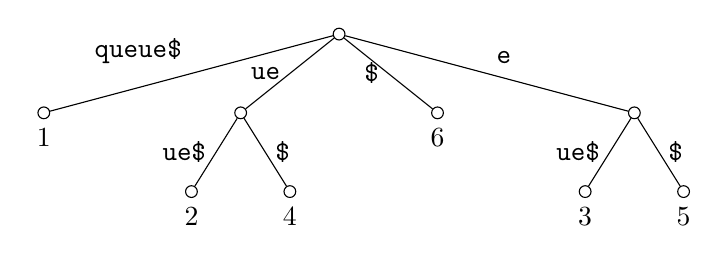
\begin{tikzpicture}[
            level distance=1cm,
            level 1/.style={sibling distance=2.5cm},
            level 2/.style={sibling distance=1.25cm},
            level 3/.style={sibling distance=0.5cm},
        ]
            \node[circle, draw, inner sep=1.5pt] {}
            child {
                node[circle, draw, inner sep=1.5pt, label={-90:1}] {}
                edge from parent node[above left] {\texttt{queue\$}}
            }
            child {
                node[circle, draw, inner sep=1.5pt] {}
                child {
                    node[circle, draw, inner sep=1.5pt, label={-90:2}] {}
                    edge from parent node[left] {\texttt{ue\$}}
                }
                child {
                    node[circle, draw, inner sep=1.5pt, label={-90:4}] {}
                    edge from parent node[right] {\texttt{\$}}
                }
                edge from parent node[left] {\texttt{ue}}
            }            
            child {
                node[circle, draw, inner sep=1.5pt, label={-90:6}] {}
                edge from parent node[left] {\texttt{\$}}
            }
            child {
                node[circle, draw, inner sep=1.5pt] {}
                child {
                    node[circle, draw, inner sep=1.5pt, label={-90:3}] {}
                    edge from parent node[left] {\texttt{ue\$}}
                }
                child {
                    node[circle, draw, inner sep=1.5pt, label={-90:5}] {}
                    edge from parent node[right] {\texttt{\$}}
                }
                edge from parent node[above right] {\texttt{e}}
            };
        \end{tikzpicture}
    \end{figure}    
    \noindent This is a much more efficient representation since we do not need to store a node for each letter. In this case, the number of nodes is $O(n)$, whereas for the suffix trie, it was $O(n^2)$.

    Now, we define the suffix tree for some string $S$. We first append $\$$ to the string and construct all the suffixes that satisfy the following properties:
    \begin{itemize}
        \item each edge has a string label;
        \item all branch nodes have at most 2 children;
        \item no two children of a branch node have two edges that started with the same character;
        \item there is a bijection between the leaf nodes and the suffixes, i.e. we can descend from the root to a leaf to recover the suffix. The entire label (from root to a node) is called its \emph{path label}.
    \end{itemize}

    In a suffix tree, there are $n+1$ suffixes, so $n+1$ leaf nodes. Also, the number of branch nodes is at most $n$. To see this, assume that we have $x$ edges, $n$ leaf nodes and $b$ branches. Then, $x = b + n - 1$- we have an edge going to each branch node and leaf node, except for the root. Moreover, since every branch node has at least 2 children, $x \geq 2b$. Hence, $b \leq n - 1$. Hence, there are $O(n)$ nodes in total. This is an improvement from suffix tries, which have $O(n^2)$ nodes.
    
    However, the suffix tree still has $O(n^2)$ space complexity- we need linear space to store the entire suffix. To mitigate this, we just store the index of the start and the end of the substring in the text. So, the suffix tree for \texttt{queue} is the following:    
    \begin{figure}[H]
        \centering
        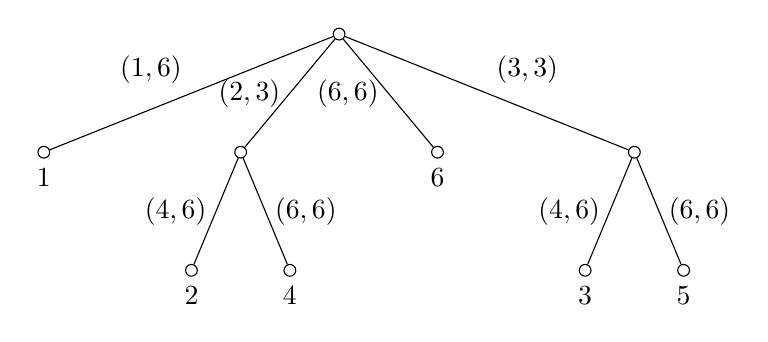
\begin{tikzpicture}[
            level distance=1.5cm,
            level 1/.style={sibling distance=2.5cm},
            level 2/.style={sibling distance=1.25cm},
            level 3/.style={sibling distance=0.5cm},
        ]
            \node[circle, draw, inner sep=1.5pt] {}
            child {
                node[circle, draw, inner sep=1.5pt, label={-90:1}] {}
                edge from parent node[above left] {$(1, 6)$}
            }
            child {
                node[circle, draw, inner sep=1.5pt] {}
                child {
                    node[circle, draw, inner sep=1.5pt, label={-90:2}] {}
                    edge from parent node[left] {$(4, 6)$}
                }
                child {
                    node[circle, draw, inner sep=1.5pt, label={-90:4}] {}
                    edge from parent node[right] {$(6, 6)$}
                }
                edge from parent node[left] {$(2, 3)$}
            }            
            child {
                node[circle, draw, inner sep=1.5pt, label={-90:6}] {}
                edge from parent node[left] {$(6, 6)$}
            }
            child {
                node[circle, draw, inner sep=1.5pt] {}
                child {
                    node[circle, draw, inner sep=1.5pt, label={-90:3}] {}
                    edge from parent node[left] {$(4, 6)$}
                }
                child {
                    node[circle, draw, inner sep=1.5pt, label={-90:5}] {}
                    edge from parent node[right] {$(6, 6)$}
                }
                edge from parent node[above right] {$(3, 3)$}
            };
        \end{tikzpicture}
    \end{figure}
    \noindent Each label now takes $O(1)$ space, so the total complexity is $O(n)$ space. We call this representation the \emph{suffix tree with short edge labels}, and the one above as the \emph{suffix tree with full edge labels}.

    One way to construct the suffix tree with short edge labels is to create the suffix trie, use it to construct the suffix tree with full edge labels by collapsing unary branches, and then replace the full edge labels with short edge labels. This is not the most efficient approach since we do need $O(n^2)$ space during the algorithm.

    A more efficient approach would involve directly constructing the suffix tree with short edge labels. We illustrate this with an example, by constructing the suffix tree with full edge labels for \texttt{queue}. We will use full edge labels for illustration purposes; the algorithm would instead make use of the short edge labels. We start by inserting the suffix \texttt{queue\$}.
    \begin{figure}[H]
        \centering
        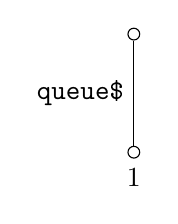
\begin{tikzpicture}[
            level distance=1.5cm,
            level 1/.style={sibling distance=2.5cm},
            level 2/.style={sibling distance=1.25cm},
            level 3/.style={sibling distance=0.5cm},
        ]
            \node[circle, draw, inner sep=1.5pt] {}
            child {
                node[circle, draw, inner sep=1.5pt, label={-90:1}] {}
                edge from parent node[left] {\texttt{queue\$}}
            };
        \end{tikzpicture}
    \end{figure}
    \noindent We insert the suffix by branching from the root. We can do the same thing when inserting the next two suffixes- \texttt{ueue\$} and \texttt{eue\$}.
    \begin{figure}[H]
        \centering
        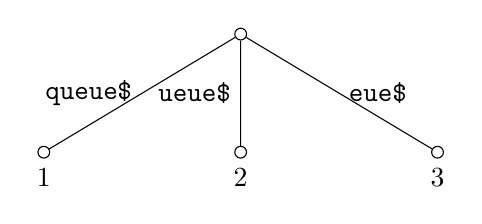
\begin{tikzpicture}[
            level distance=1.5cm,
            level 1/.style={sibling distance=2.5cm},
            level 2/.style={sibling distance=1.25cm},
            level 3/.style={sibling distance=0.5cm},
        ]
            \node[circle, draw, inner sep=1.5pt] {}
            child {
                node[circle, draw, inner sep=1.5pt, label={-90:1}] {}
                edge from parent node[left] {\texttt{queue\$}}
            }
            child {
                node[circle, draw, inner sep=1.5pt, label={-90:2}] {}
                edge from parent node[left] {\texttt{ueue\$}}
            }
            child {
                node[circle, draw, inner sep=1.5pt, label={-90:3}] {}
                edge from parent node[right] {\texttt{eue\$}}
            };
        \end{tikzpicture}
    \end{figure}
    \noindent At this point, the next suffix is \texttt{ue\$}. We already have a node starting with \texttt{ue}, but this is not a complete match (i.e. the branch has a longer label). So, we perform an \emph{edge-split} first to ensure we can branch at the right position.
    \begin{figure}[H]
        \centering
        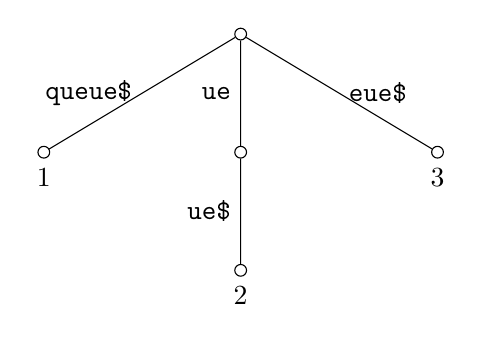
\begin{tikzpicture}[
            level distance=1.5cm,
            level 1/.style={sibling distance=2.5cm},
            level 2/.style={sibling distance=1.25cm},
            level 3/.style={sibling distance=0.5cm},
        ]
            \node[circle, draw, inner sep=1.5pt] {}
            child {
                node[circle, draw, inner sep=1.5pt, label={-90:1}] {}
                edge from parent node[left] {\texttt{queue\$}}
            }
            child {
                node[circle, draw, inner sep=1.5pt] {}
                child {
                    node[circle, draw, inner sep=1.5pt, label={-90:2}] {}
                    edge from parent node[left] {\texttt{ue\$}}
                }
                edge from parent node[left] {\texttt{ue}}
            }
            child {
                node[circle, draw, inner sep=1.5pt, label={-90:3}] {}
                edge from parent node[right] {\texttt{eue\$}}
            };
        \end{tikzpicture}
    \end{figure}
    \noindent We can now insert \texttt{ue\$} as a child of the branch \texttt{ue}.    
    \begin{figure}[H]
        \centering
        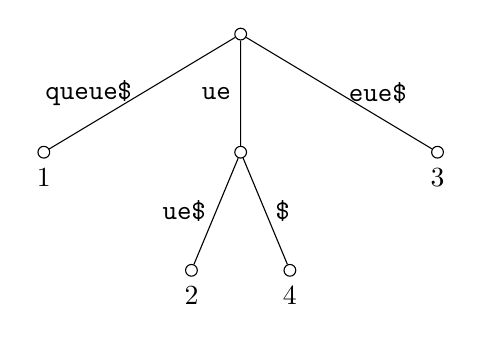
\begin{tikzpicture}[
            level distance=1.5cm,
            level 1/.style={sibling distance=2.5cm},
            level 2/.style={sibling distance=1.25cm},
            level 3/.style={sibling distance=0.5cm},
        ]
            \node[circle, draw, inner sep=1.5pt] {}
            child {
                node[circle, draw, inner sep=1.5pt, label={-90:1}] {}
                edge from parent node[left] {\texttt{queue\$}}
            }
            child {
                node[circle, draw, inner sep=1.5pt] {}
                child {
                    node[circle, draw, inner sep=1.5pt, label={-90:2}] {}
                    edge from parent node[left] {\texttt{ue\$}}
                }                
                child {
                    node[circle, draw, inner sep=1.5pt, label={-90:4}] {}
                    edge from parent node[right] {\texttt{\$}}
                }
                edge from parent node[left] {\texttt{ue}}
            }
            child {
                node[circle, draw, inner sep=1.5pt, label={-90:3}] {}
                edge from parent node[right] {\texttt{eue\$}}
            };
        \end{tikzpicture}
    \end{figure}
    \noindent We have to do the same thing when inserting \texttt{e\$}- we edge-split \texttt{eue\$}.    
    \begin{figure}[H]
        \centering
        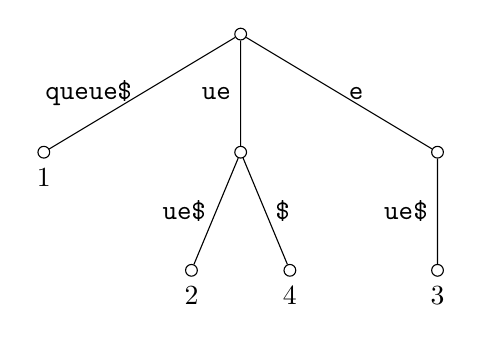
\begin{tikzpicture}[
            level distance=1.5cm,
            level 1/.style={sibling distance=2.5cm},
            level 2/.style={sibling distance=1.25cm},
            level 3/.style={sibling distance=0.5cm},
        ]
            \node[circle, draw, inner sep=1.5pt] {}
            child {
                node[circle, draw, inner sep=1.5pt, label={-90:1}] {}
                edge from parent node[left] {\texttt{queue\$}}
            }
            child {
                node[circle, draw, inner sep=1.5pt] {}
                child {
                    node[circle, draw, inner sep=1.5pt, label={-90:2}] {}
                    edge from parent node[left] {\texttt{ue\$}}
                }                
                child {
                    node[circle, draw, inner sep=1.5pt, label={-90:4}] {}
                    edge from parent node[right] {\texttt{\$}}
                }
                edge from parent node[left] {\texttt{ue}}
            }
            child {
                node[circle, draw, inner sep=1.5pt] {}
                child {
                    node[circle, draw, inner sep=1.5pt, label={-90:3}] {}
                    edge from parent node[left] {\texttt{ue\$}}
                }
                edge from parent node[right] {\texttt{e}}
            };
        \end{tikzpicture}
    \end{figure}
    \noindent We can now insert \texttt{e\$} to the tree.
    \begin{figure}[H]
        \centering
        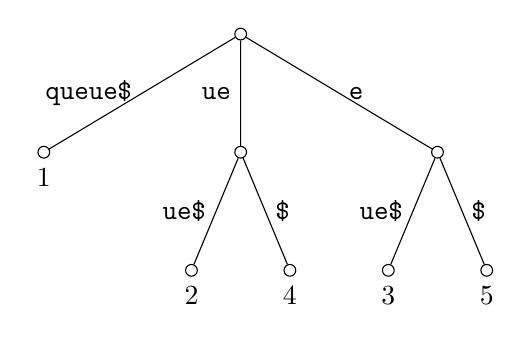
\begin{tikzpicture}[
            level distance=1.5cm,
            level 1/.style={sibling distance=2.5cm},
            level 2/.style={sibling distance=1.25cm},
            level 3/.style={sibling distance=0.5cm},
        ]
            \node[circle, draw, inner sep=1.5pt] {}
            child {
                node[circle, draw, inner sep=1.5pt, label={-90:1}] {}
                edge from parent node[left] {\texttt{queue\$}}
            }
            child {
                node[circle, draw, inner sep=1.5pt] {}
                child {
                    node[circle, draw, inner sep=1.5pt, label={-90:2}] {}
                    edge from parent node[left] {\texttt{ue\$}}
                }                
                child {
                    node[circle, draw, inner sep=1.5pt, label={-90:4}] {}
                    edge from parent node[right] {\texttt{\$}}
                }
                edge from parent node[left] {\texttt{ue}}
            }
            child {
                node[circle, draw, inner sep=1.5pt] {}
                child {
                    node[circle, draw, inner sep=1.5pt, label={-90:3}] {}
                    edge from parent node[left] {\texttt{ue\$}}
                }
                child {
                    node[circle, draw, inner sep=1.5pt, label={-90:5}] {}
                    edge from parent node[right] {\texttt{\$}}
                }
                edge from parent node[right] {\texttt{e}}
            };
        \end{tikzpicture}
    \end{figure}
    \noindent Next, we insert \texttt{\$}.
    \begin{figure}[H]
        \centering
        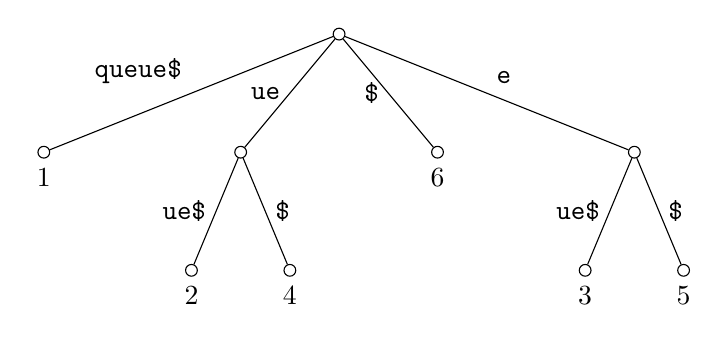
\begin{tikzpicture}[
            level distance=1.5cm,
            level 1/.style={sibling distance=2.5cm},
            level 2/.style={sibling distance=1.25cm},
            level 3/.style={sibling distance=0.5cm},
        ]
            \node[circle, draw, inner sep=1.5pt] {}
            child {
                node[circle, draw, inner sep=1.5pt, label={-90:1}] {}
                edge from parent node[above left] {\texttt{queue\$}}
            }
            child {
                node[circle, draw, inner sep=1.5pt] {}
                child {
                    node[circle, draw, inner sep=1.5pt, label={-90:2}] {}
                    edge from parent node[left] {\texttt{ue\$}}
                }
                child {
                    node[circle, draw, inner sep=1.5pt, label={-90:4}] {}
                    edge from parent node[right] {\texttt{\$}}
                }
                edge from parent node[left] {\texttt{ue}}
            }            
            child {
                node[circle, draw, inner sep=1.5pt, label={-90:6}] {}
                edge from parent node[left] {\texttt{\$}}
            }
            child {
                node[circle, draw, inner sep=1.5pt] {}
                child {
                    node[circle, draw, inner sep=1.5pt, label={-90:3}] {}
                    edge from parent node[left] {\texttt{ue\$}}
                }
                child {
                    node[circle, draw, inner sep=1.5pt, label={-90:5}] {}
                    edge from parent node[right] {\texttt{\$}}
                }
                edge from parent node[above right] {\texttt{e}}
            };
        \end{tikzpicture}
    \end{figure}
    \noindent The suffix tree is now complete.

    This algorithm takes $O(n)$ space complexity, but has worst-case complexity $O(n^2)$, e.g. if we have to edge-split every time. The average case is $O(n \log n)$. There are more efficient algorithms that require $O(n)$ time complexity.

    We will now use the suffix tree for different string algorithms. If we have a string $S$ and a substring $T$ to search in the string, we construct a tree on $S$, and then match each letter in $T$ with the corresponding node. If we cannot match $T$ completely, then the string is not present. If it is present, we can return the index of the match by using the branch node we are at. This algorithm is very similar to the one for suffix tries we saw above. The time taken for this algorithm is linear with respect to the substring. We can also find all occurrences using this approach.

    Now, we try to find the longest repeated substring in a text $S$. We can construct the suffix tree for $S$ in $O(n)$ time. We then traverse the tree to find the branch node with the greatest string depth. A branch node corresponds to a common substring, and the string depth keeps track of the length of the common substring. We can traverse in $O(n)$ time, so the entire algorithm is $O(n)$.

    Next, we can find a longest common substring of texts $S$ and $T$. To do so, we construct the suffix tree for $S\#T\$$, where $\#$ and $\$$ are symbols not in $\Sigma$. This is called the \emph{generalised suffix tree}. We then traverse the tree in a similar way as the longest repeated substring, but we are looking for a common branch node with the greatest string depth. A common branch is one that has leaf nodes corresponding to suffix starting in both $S$ and $T$.

    Now, we will look at a method to identify common branch nodes. For each branch node $v$, we keep track of two values- whether it has a leaf node with suffix value corresponding to a string in $S$ ($b_1(v)$), and whether it has a leaf node with suffix value corresponding to a string in $T$ ($b_2(v)$). Then, $v$ is a branch node if and only if $b_1(v) \land b_2(v)$. We can compute the $b_i(v)$ values as follows:
    \begin{itemize}
        \item if $v$ is a leaf node, then we can check the value of the suffix to compute $b_i(v)$- $b_1(v)$ is \texttt{true} if $1 \leq j \leq m$ and $b_2(v)$ is \texttt{true} if $m+2 \leq j \leq m+n+1$, where $m$ and $n$ are the lengths of $S$ and $T$ respectively;
        \item instead, if $v$ is a branch node, then $b_i(v) = b_i(w_1) \land b_i(w_2) \land \dots \land b_i(w_n)$, where $w_1, w_2, \dots, w_n$ are the descendant leaf nodes of $v$. 
    \end{itemize}

    So, the algorithm for longest common substring is the following:
    \begin{itemize}
        \item build the generalised suffix tree;
        \item calculate the values $b_i(v)$ for every node $v$;
        \item find the common branch node with maximum string depth.
    \end{itemize}
    The last 2 steps can be combined. Each step takes $O(m+n)$ time, so the algorithm overall takes $O(m+n)$ time.

    We will now illustrate that the character $\#$ is required in order to correctly output the result. So, assume that the two strings are \texttt{a} and \texttt{bab}. Then, the suffix tree for $ST\$$ is the following:
    \begin{figure}[H]
        \centering
        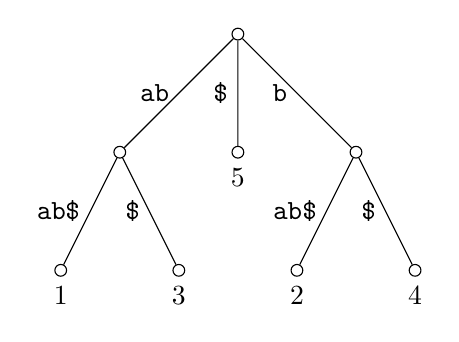
\begin{tikzpicture}
            \node[circle, draw, inner sep=1.5pt] {}
            child {
                node[circle, draw, inner sep=1.5pt] {}
                child {
                    node[circle, draw, inner sep=1.5pt, label={-90:1}] {}
                    edge from parent node[left] {\texttt{ab\$}}
                }
                child {
                    node[circle, draw, inner sep=1.5pt, label={-90:3}] {}
                    edge from parent node[left] {\texttt{\$}}
                }
                edge from parent node[left] {\texttt{ab}}
            }
            child {
                node[circle, draw, inner sep=1.5pt, label={-90:5}] {}
                edge from parent node[left] {\texttt{\$}}
            }
            child {
                node[circle, draw, inner sep=1.5pt] {}
                child {
                    node[circle, draw, inner sep=1.5pt, label={-90:2}] {}
                    edge from parent node[left] {\texttt{ab\$}}
                }
                child {
                    node[circle, draw, inner sep=1.5pt, label={-90:4}] {}
                    edge from parent node[left] {\texttt{\$}}
                }
                edge from parent node[left] {\texttt{b}}
            };
        \end{tikzpicture}
    \end{figure}
    \noindent Here, the common branch node with the greatest depth is \texttt{ab}. However, it is not a common substring of \texttt{a} and \texttt{bab}.
\end{document}